\chapter{Optics II: Applications of Lenses}
\section{Introduction}
In this experiment, we will apply our knowledge of lenses and geometrical optics to build a microscope and telescope. Microscopes are common in the medical field, and allow doctors to closely examine things that our eyes cannot resolve. Understanding the basic operation is important to knowing when they are useful, and how they can be improved. Telescopes allow a user to view a far away object as if it were closer, again allowing us to resolve details that the naked eye cannot. Both devices are useful in a wide variety of fields. Throughout this experiment, we will be using the `thin lens' approximation\footnote{Many approximations are made with ``thin lenses''. However, even the most sophisticated treatments of optics usually begin with these ``thin lens approximations''.}. 

\section{Theory}
Why do we need optical instruments? The human eye is incredible in its ability to capture a wide range of colors and focus over a wide range of distances. However, there are some objects that are either too small, or too far away for the eye to resolve. Doctors and scientists require optical instruments to take improve our natural ability.

\subsection{The Near Point}
In the human eye, light is focused on the retina by the elastic lens. Though the lens can change its focal length (through contractions of the ciliary muscles), the range of focus is limited. The closest point at which the eye can get a sharp image of an object is called the near point. The near point is different for every person, but the value of $25\, \textrm{cm}$ is an average over a random segment of the population. We use the standard reference of $25\, \textrm{cm}$ here. Young people with good eyesight may have a near point as close as $10-15\, \textrm{cm}$, and very young children have an even smaller one. You will determine the near point for your eyes in the course of this experiment.

\subsection{Resolution}
In art museums, you probably observed the following effect. As you look at an impressionist painting from a distance, the picture appears sharp and easily identifiable. But as you approach the picture, you observe that it is made up of a number of smaller objects, large dots or blobs, and is quite coarse-grained.\myskip

What happened? Your retina consists of an array of light receptors, somewhat like the pixels in a video camera. When you are far enough away from the picture, all light rays from an object like a big dot fall onto a single receptor. Your visual impression from a long distance therefore consists of various sharp points. As you approach the picture, rays from this object begin to strike several receptors and you recognize that the blob is an extended object. If you look at the same picture, but shrunk by a factor of 10, you observe that you can get much closer before seeing the individual blobs. Such effects are related to the resolution limits of the eye.\myskip

The figure on the next page illustrates how an image appears on the retina. Note that the image is inverted on the retina. We actually �see� objects upside down. (Our brains do the work of inverting it back!) When we view an object, its size is determined by how big the object�s image is on our retina. \myskip

Figure \ref{fig:resolution} below, we see that the size of the retinal image is directly proportional to $\tan\alpha=h/s$. Clearly, there is a minimum value of $\alpha$ that can be resolved on the retina. 
\begin{figure}[h]
\centering
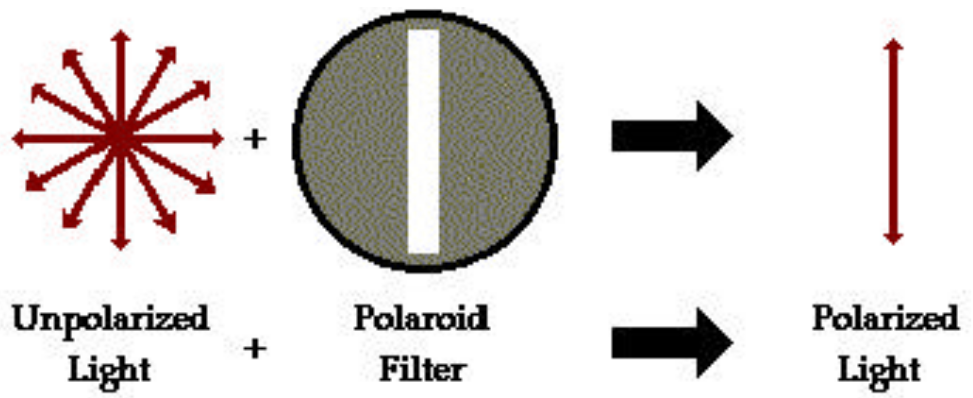
\includegraphics[width=0.8\textwidth]{./Exp7/pic/image1.png}
\caption{The Formation of Images on the Retina}
\label{fig:resolution}
\end{figure} 


\subsection{Need for Magnification}

Suppose a person with a near point of $25\, \textrm{cm}$ examines the object shown in the figure above. To see the most detail, the person should view the object so that it appears to be as large as possible while remaining in focus. As discussed above, the size of the retinal image varies as $\tan\alpha=h/s$. This means that the retinal image gets larger as s gets smaller (i.e., as the object is brought closer to the eye). The largest focused image this person can see is obtained when $s = 25\, \textrm{cm}$. The size of the object when viewed at $25\, \textrm{cm}$ is \underline{defined} to have a magnification of unity. Is there any way to see more detail on the object, or, equivalently, can the object be made to appear larger? The answer is yes, and the simplest means of making the object appear larger is to use a magnifying glass.

\subsection{Virtual Images vs. Real Images}
\label{sec:vimages}

In the lens experiments we have been covering so far, it has been possible to place a screen at the location of the image and since the light rays focus at that screen, a clear image is formed on the screen. Such images are real. However, consider a ray diagram with a lens, where the object is placed between the focal point and the lens, as in Figure \ref{fig:virtualimage}.

\begin{figure}[h]
\centering
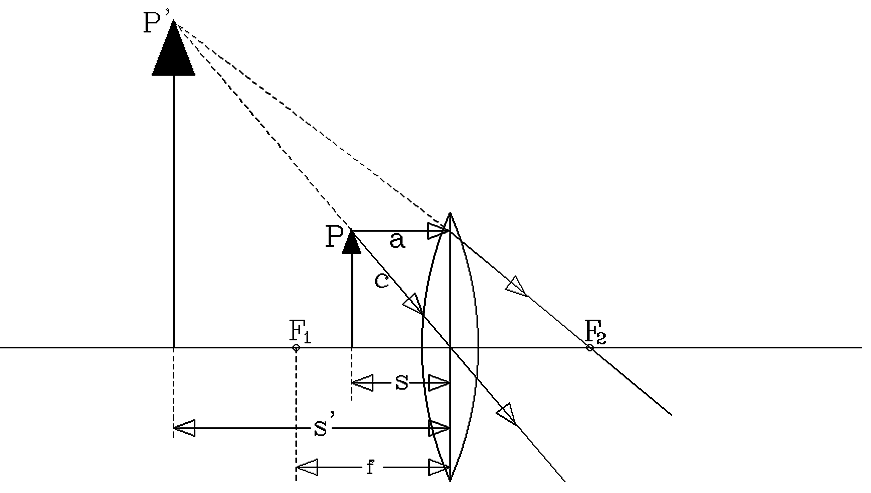
\includegraphics[width=0.7\textwidth]{./Exp7/pic/image5.png}
\caption{Convergent Lens: Virtual Image}
\label{fig:virtualimage}
\end{figure} 

  When the object is placed exactly at the focal point, the rays exit parallel (and the image is infinitely far away). (Remember that this is how we define the focal point, and how we determined the focal length in Experiment 4)  As the object gets even closer to the lens, as shown in Figure \ref{fig:virtualimage}, the rays must diverge as they exit. If you extend the outgoing rays backward (behind the lens), you find that they intersect behind the original object. A virtual image is formed. It cannot be captured on a screen, but you can see it as you look through the lens - the object appears at the position of the virtual image and enlarged.
  
  This same phenomena happens when you look into a mirror and see a clear reflection of yourself. The rays originating from your body never really converge, so it is not possible to see the image on a screen.

\subsection{Parallax}

In everyday life, we are able to tell distance by a combination of seeing how large things are relative to other objects, and how they move relative to each other. But what happens when we are not sure what the size of an object is supposed to be? In optics experiments, both virtual and real images can be magnified in non-intuitive ways, so using the size of the image we see compared to the original object is not a good way to tell which object is closer or further. We must use the method of parallax. Parallax is the apparent change in distance between to objects that depends on where the observer is.\myskip

Imagine walking along a road and seeing two trees in the distance, as in Figure \ref{fig:parallax}. At point A in the left image, you see an apparent distance between the two trees given by L$_A$. But as you walk to point B, you would notice that that distance changes dramatically, and the trees only look lined up when you are standing directly in front of them. However, if the trees are in nearly the same location, the apparent change between  L$_A$ and L$_B$ is very small as you walk along the road.\myskip

\begin{figure}[h]
\centering
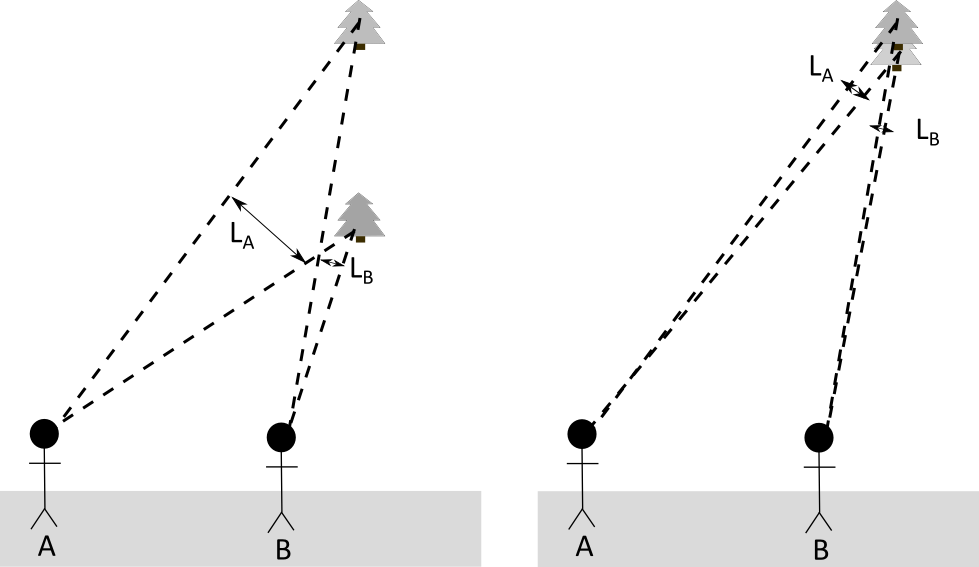
\includegraphics[width=0.7\textwidth]{./Exp7/pic/image_parallax.png}
\caption{An example of parallax. In the image on the left, the difference in observed distance between the trees changes dramatically as you move along the road, hence the large difference between L$_A$ and L$_B$. In the image on the right, where the trees are nearly in the same location,  L$_A$ and L$_B$ are basically unchanged.}
\label{fig:parallax}
\end{figure} 


\subsection{The Magnifying Glass}

A magnifying glass is a simple converging lens with short focal length that can make an object�s image on the retina larger. How does it work? One limitation to the detail you see on an object is the limited angular resolution, which is due to the limited size of the individual receptors. (There is nothing we can do about this.) But the other limitation is that we cannot make the retinal image larger by bringing the object closer than the near point. There is a way to overcome this limitation, and it is used in all optical magnifying devices.\myskip

Consider the object and lens of focal length $f$ shown in Figure \ref{fig:virtualinf}. 
\begin{figure}[h]
\centering
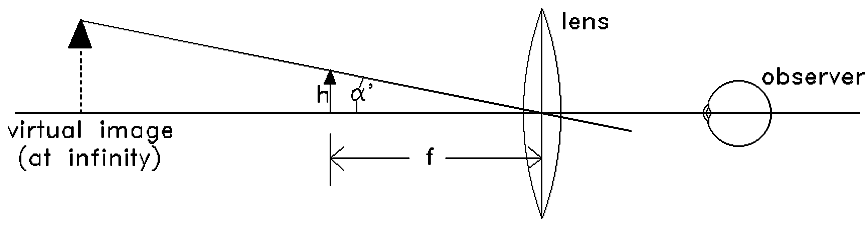
\includegraphics[width=0.8\textwidth]{./Exp7/pic/image2.png}
\caption{Virtual Image at infinity}
\label{fig:virtualinf}
\end{figure} 

The object is placed a focal length $f$ away from the lens. Using the lens equation, we find that a virtual image is formed at infinity as shown. (If you feel uncomfortable thinking of an image at infinity, you might prefer to think of it as simply a very large distance.)\myskip

If the rays of light from the ends of the object that pass through the center of the lens are extended to the left, they also pass through the ends of the image. (If this is not obvious, return to Experiment 1-5 and review the rules for ray tracing). This means that the angle $\alpha'=\tan^{-1}h/f$ is the same for both the object and the virtual image. Remember what an image represents - looking at the object through the lens can be represented as looking directly at the image. Since the image is very far away, its size does not appear to change as the eye (to the right of the lens) is moved small distances back and forth. \myskip

What actually happened when you put the converging lens one focal length in front of the object? The rays leaving the lens that actually hit the eye (not the ray shown in the figure) will be nearly parallel and therefore the rays appear to come from an infinitely far object � unless you are near-sighted, your eye can totally relax. \myskip

When we view the image, its size is proportional to $\tan\alpha'=h/f$. The \emph{angular magnification} of the magnifying glass is defined as:
\begin{equation}
  M=\frac{\tan\alpha'}{\tan\alpha}=\frac{h/f}{h/25\ \mathrm{cm}}=\frac{25\ \mathrm{cm}}{f\ \mathrm{cm}}
\end{equation}

The \textbf{magnification $M$} represents the ratio of the \underline{apparent} size of the object when viewed using the magnifying glass to that of the object when viewed directly at a distance of $25\, \textrm{cm}$.\myskip

If $f$ is less than $25\, \textrm{cm}$, the lens increases the apparent size of the object and permits you to see more detail. Viewing an object with a magnifying glass of focal length $12.5\, \textrm{cm}$ produces a retinal image twice as large as that formed when the object is viewed directly $25\, \textrm{cm}$ away.\myskip

If a lens of focal length $25\, \textrm{cm}$ is used as a magnifying glass, the apparent size of the object is the \underline{same} as that seen when looking directly at the object $25\, \textrm{cm}$ from the eye. Using the lens, however, permits your eye to relax because it views parallel rays, just as if the object were located very far away.\myskip

In practice, one does not always place the object at the focal point of the magnifying glass, but it is at that point that the magnification is greatest. Magnification can also be equivalently defined as the ratio of the height of the image to that of the object. By drawing congruent triangles, it should be clear that this implies that 
$$
M= \frac{h_i}{h_o} = \frac{-s_i}{s_o}
$$

Note that we follow the sign conventions used in the course textbook here - you may wish to review Section 34-7 of Fundamentals of Physics.

\subsection{The Microscope}
\label{sec:theorym}
For various reasons, a single lens magnifier (such as a magnifying glass) can only provide good images with relatively small magnifications. To achieve higher magnification, a device known as a compound microscope can be used. \myskip

A compound microscope employs two lenses as shown in the next figure. The object to be viewed is placed at a distance $s_{o1}$, just beyond the focal length, $F$, of the first lens, called the objective lens. The light collected by the objective lens forms a real (enlarged) image of the object at $s_{i1}$. (The image is real because a screen placed at $s_{i1}$ would display an actual inverted image of the object.) The second lens, the eyepiece, has a focal length $f$ and acts as a magnifying glass that is used to examine the image $s_{i1}$. The position of the image formed by the first lens becomes the object for the second lens, and the distance $s_{o2}$ is defined as in Fig. \ref{fig:micro1}. Adjusting the position of the eyepiece adjusts the position of the final image. \myskip

As discussed in the preceding section, the observer looking through the eyepiece (magnifier) sees a virtual image $s_{i2}$ of the real image.
\begin{figure}[h]
\centering
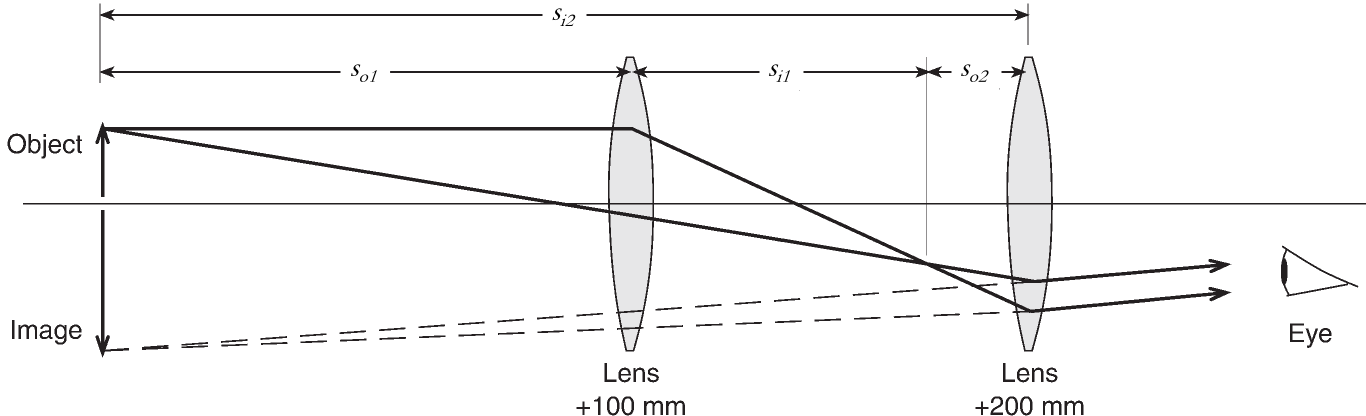
\includegraphics[width=0.8\textwidth]{./Exp7/pic/image9a.png}
\caption{A Compound Microscope}
\label{fig:micro1}
\end{figure} 

How big does the original object appear? Since magnification represents a multiplicative factor, we simply have to calculate the magnification of the original image $I_1$, by the first lens, then multiply that by the magnification of the second lens. \myskip

The total magnification of the microscope is then:
\begin{equation}
	M=M_{eyepiece}M_{objective} =  \left(\frac{-s_{i1}}{s_{o1}}\right) \left(\frac{-s_{i2}}{s_{o2}}\right)
\end{equation}

\subsection{The Telescope}
\label{sec:telescope}
The optical system of a refracting telescope has the same elements as those of a compound microscope. In both instruments, the real image formed by an \underline{objective} lens is viewed through an \underline{eyepiece}. However, the object of a telescope is distant, the incoming rays are (approximately) parallel and the objective lens forms the first image $I_1$, near its focal point $F$, as shown in the figure below. (By contrast, for the microscope $s'\gg F$.)\myskip
\begin{figure}[h]
\centering
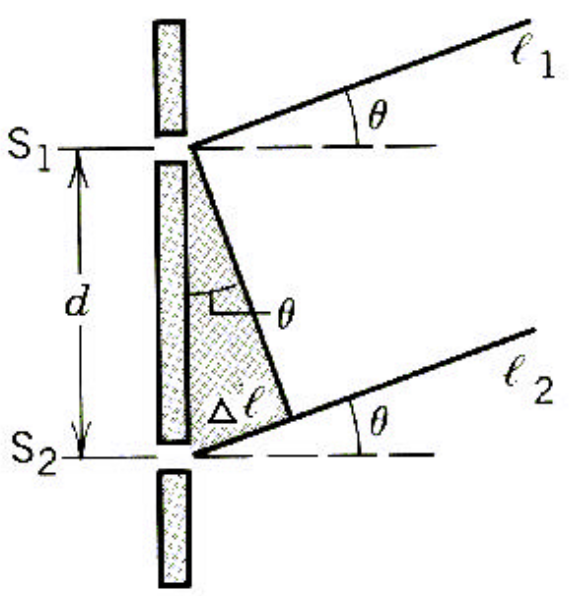
\includegraphics[width=0.8\textwidth]{./Exp7/pic/image4.png}
\caption{Telescope}
\end{figure} 

\textbf{The important point here is that although the object is very far away, it still subtends a small angle in our naked eye (otherwise we wouldn't be able to see it)}. The assumption that it is very far away is to make sure that there will be an image $I_1$ at the focal point of the objective lens, which again serves as the object for the eyepiece. In order for $I_2$ -- the final virtual image made by the eyepiece -- to be near infinity (for relaxed viewing), the eyepiece needs to be located so that $I_1$ is also near its focal point $f$. Therefore, the distance between the objective lens and the eyepiece -- the length of the telescope -- is the sum of the focal lengths $F+f$.\myskip

The angular magnification of the telescope is easily derived by noting that $\alpha$, the very small angle that the distant object would subtend for the \underline{unaided eye}, is essentially the same as the angle subtended by the image $I_1$ from the objective lens. Then from the figure above we have:
\begin{equation}
  \tan a=\frac{y}{F}
\end{equation}
and angle $A$, subtended by $I_1$ at the eyepiece, we have:
\begin{equation}
  \tan A =\frac{y}{f}
\end{equation}
so:
\begin{align}
  M_{\mathrm{telescope}}&=\frac{\tan A}{\tan a}=\frac{y/f}{y/F}\\
  M_{\mathrm{telescope}}&=\frac{F}{f}
\end{align}


\section{Experiments}


\subsection{The Near Point}


In the first part of the lab, you will measure the near point of each eye. Tape the paper grid pattern onto the screen and place the screen on the optical bench. Place your head so that one eye is at the end of the  optical bench. Move the screen as close to your eye as possible, consistent with the requirement that the screen remains in focus. The distance s is the near point for that eye. Repeat for the other eye.
\begin{itemize}
\item Is the near point the same for both eyes?
\item How do these values for your eyes compare to the standard value of $25\, \textrm{cm}$?
\end{itemize}

If the values you obtain are different from the conventional $25\, \textrm{cm}$ value, it should not be surprising; as you compare your values other people in the class, you will probably see a wide variation. So as to make quantitative comparisons of the instruments that we will be using in the following sections, we use a standardized reference near point of $25\, \textrm{cm}$. We choose this value since the �average� person cannot get closer to an object than this and still keep it in focus.

\subsection{Virtual Images}

In this part of the lab, we will study virtual images formed by concave lenses. Concave lenses have negative focal lengths, and are therefore sometimes referred to as ``diverging lenses''. You will then use
another lens to form a real image of the virtual image. In this way you can identify the
location of the virtual image.\myskip

Set up the -150 mm lens and light source as in Fig. \ref{virt1}, with the crossed arrow object on the light source pointing towards the lens.

\begin{figure}[h]
\centering
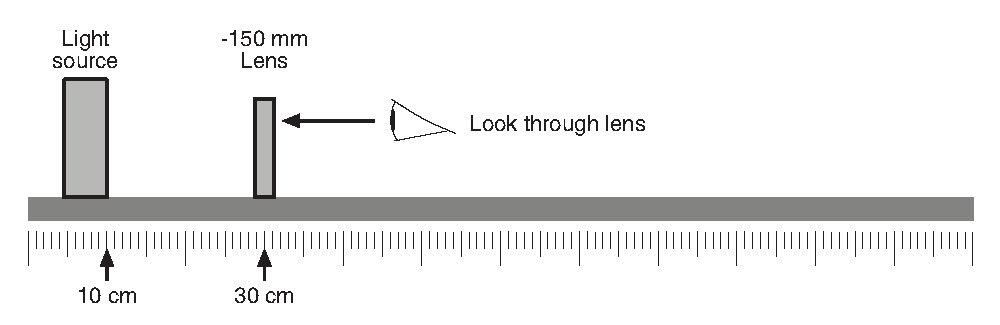
\includegraphics[width=0.7\textwidth]{./Exp7/pic/virtual-1.png}
\caption{Virtual Image set-up}
\label{virt1}
\end{figure} 

\begin{itemize}
\item Look through the lens toward the light source. Describe the
image. Is it upright or inverted? Does it appear to be larger or smaller than the
object?

\item Which do you think is closer to the lens: the image or the object? Why do you
think so?

\item Using the lens equation (see Experiment 2-6, and also on the next page) and remembering that the concave lens has a negative focal length, calculate the position of the virtual image.
\end{itemize}

Place the +200 mm lens anywhere between 50 cm and 80 cm on the optical bench and then move the screen so that the image is focused (Fig. \ref{virt2}).
\begin{figure}[h]
\centering
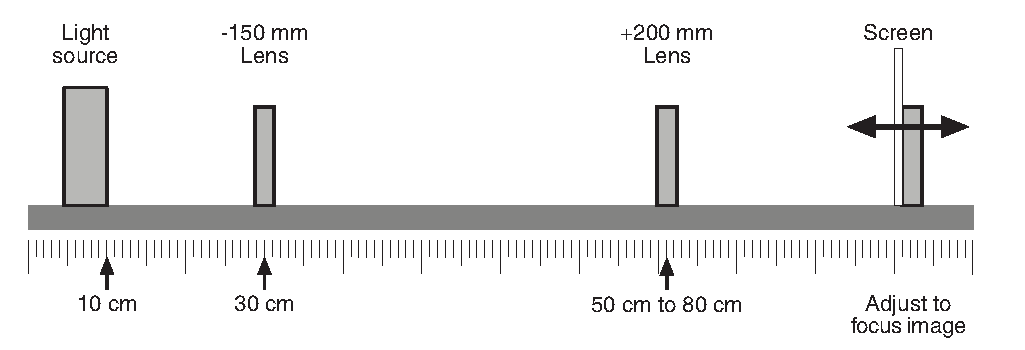
\includegraphics[width=0.7\textwidth]{./Exp7/pic/virtual-2.png}
\caption{Placing a second lens to form a real image from the virtual one.}
\label{virt2}
\end{figure} 

\begin{itemize}
\item Why are you able to see the image on the screen? What is serving as the object?
\end{itemize}

In the following step, you will discover the location of the virtual image by replacing it with the light
source. Remove the negative lens from the bench, and note that the image on the screen goes out of focus. Slide the light source to a new position so that a clear image is formed on the screen. (Do not move the positive lens or the screen.) Make sure you write down the positions of all components. (Fig. \ref{virtu3})

\begin{figure}[h]
\centering
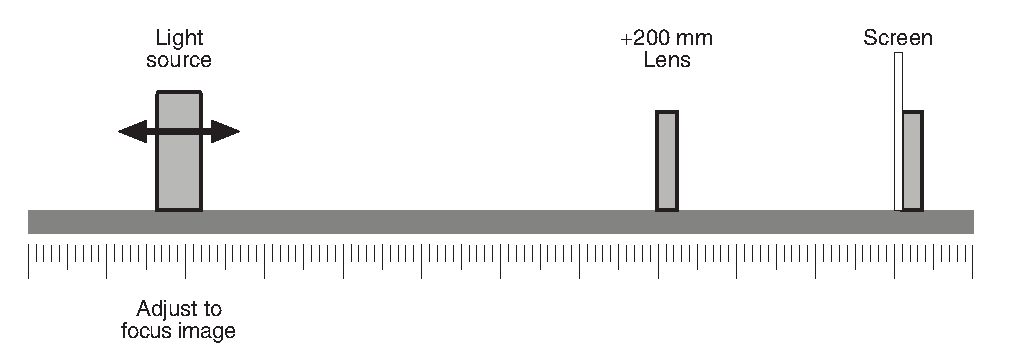
\includegraphics[width=0.7\textwidth]{./Exp7/pic/virtual-3.png}
\caption{Remove the first lens, then move the light source to the position of where the virtual image was.}
\label{virtu3}
\end{figure} 

Your light source is now at the position of the virtual image. Note that it may differ from your prediction made earlier from the thin lens equation. Why is this? (Remember the approximations made in the thin lens equation)


\subsection{The Microscope}
\myskip
\begin{figure}[h]
\centering
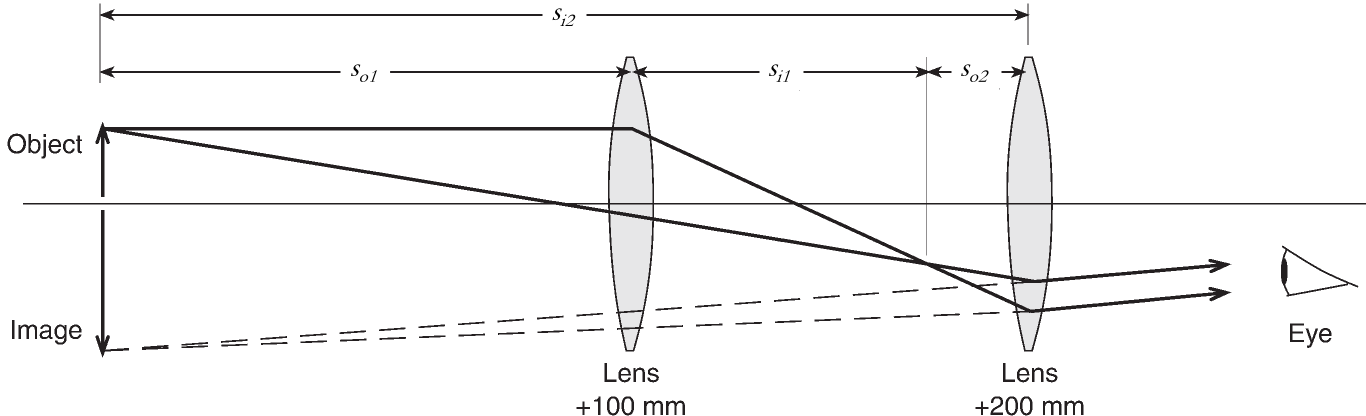
\includegraphics[width=0.8\textwidth]{./Exp7/pic/image9a.png}
\caption{Measuring the Magnification of the Microscope}
\label{fig:microscope}
\end{figure} 

%{\bf NOTE}:  you may find that the distance ($S+S'$) should be more like $50\, \textrm{cm}$ than the $35\, \textrm{cm}$ noted in the diagram.\myskip
A microscope magnifies an object that is close to the objective lens. The microscope
in this experiment will form an image in the same place as the object (see Figure
\ref{fig:microscope}). 

As discussed earlier, the magnification, M, of a two-lens system is equal to the product of the magnifications
of the individual lenses. Magnification is defined to be the negative of the ratio of the image distance to the object distance, as in the lecture course textbook. In a microscope, the eyepiece uses the image of the objective lens as its object. Therefore, the total magnification of the microscope can be given as:

\begin{equation}
\label{eq:magnification}
	M=M_{eyepiece}M_{objective} =  \left(\frac{-s_{i1}}{s_{o1}}\right) \left(\frac{-s_{i2}}{s_{o2}}\right)
\end{equation}

In this experiment, we would like to achieve a magnification of \textbf{-2} (be careful with sign conventions in the equation above).

\subsubsection*{Procedure}
First, tape the paper grid pattern to the screen to serve as an object. Then, use the 100mm lens as the objective lens and the 200mm lens as the eyepiece, as shown in Fig. \ref{fig:microscope}

The goal here is to create a real image with the objective lens, and then calculate where to place the eyepiece so that the final virtual image is at the same place as the original object.

Set up the Objective lens (f=100 mm) 30 cm away from the screen ($s_{o1}$). Given this, and the thin lens equation:
$$
\frac{1}{f}=\frac{1}{s_{o}}+\frac{1}{s_i},
$$
you can calculate where the image ($s_{i1}$)from the objective should show up. In order to measure the magnification by eye, we need to place the eyepiece so that the virtual image is formed exactly where the original object is. If we do this, then we can accurately compare the magnified grid to the unmagnified one.

 Looking at Figure \ref{fig:microscope}, we can see that the \textbf{absolute} value of $s_{i2}$, the image distance from the eyepiece, is given by:
\begin{equation}
\label{eq:sum}
s_{i2} = s_{o2}+s_{i1}+s_{o1},
\end{equation}
(Note that with our usual sign convention for object and image distances, $s_{i2}$ is actually negative.)
Plugging Equation \ref{eq:sum} into Equation \ref{eq:magnification}, we can eliminate $s_{i2}$. Now,  keeping in mind that we would like to achieve a magnification of -2, \textbf{calculate where you should place the second lens ($s_{o2}$).}

Place the eyepiece and look through your microscope. As you move your head from side to side, you should notice that there is little to no parrallax between the lines on the actual object and the lines that you see through the center of the microscope.
\begin{itemize}

\item Estimate the magnification by comparing the magnified and unmagnified grids. Quote an error and compare this to the magnification you attempted to get.

\item Is the image inverted or upright? How do you explain this?

\item Create and fill out a table like the one below in your lab report.

\end{itemize}
\begin{center}
\begin{tabular}{|l|l|}

\hline
Position of Objective Lens & \hspace{4 cm} \\ \hline
Position of Eyepiece Lens &                    \\ \hline
Position of Screen &                    \\ \hline
$s_{o1}$ & \\ \hline
$s_{i1}$ & \\ \hline
$s_{o2}$ & \\ \hline
$s_{i2}$ & \\ \hline
Observed Magnification & \\ \hline

\end{tabular}
\end{center}



\subsection{The Telescope}
As we have seen before, the telescope works on a similar principle to the microscope, except now, our object distance is effectively infinite.
\myskip
\begin{figure}[h]
\centering
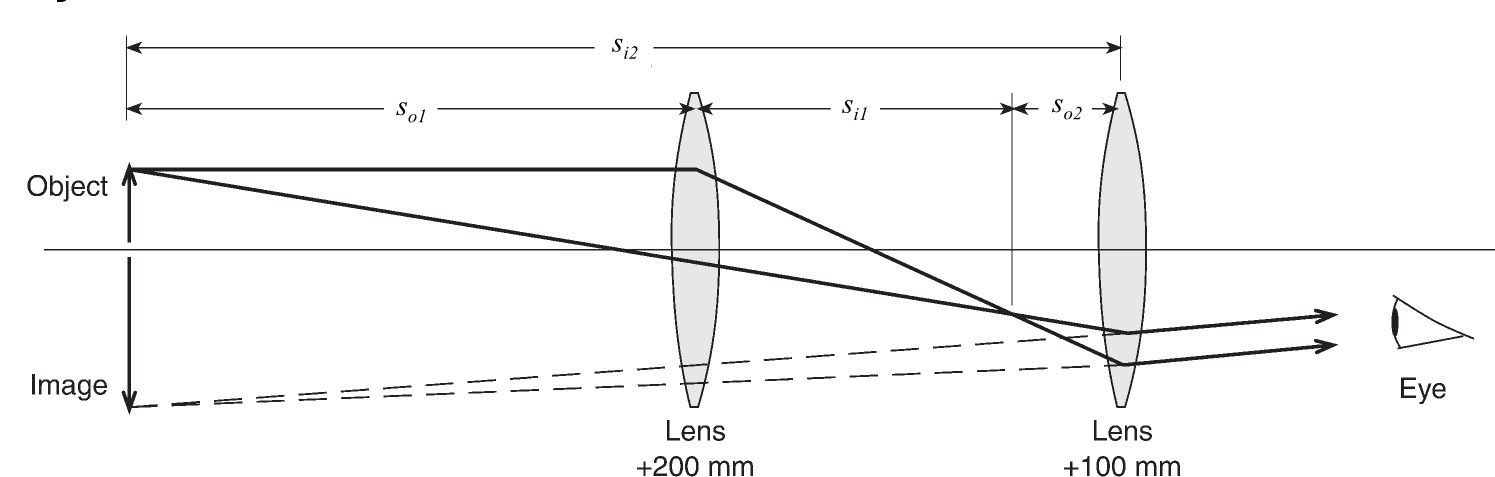
\includegraphics[width=0.8\textwidth]{./Exp7/pic/image10a.png}
\caption{Schematic of a telescope.}
\end{figure} 

We assemble a telescope and measure its magnification. Since the final object is formed near infinity, we can compare far away objects with a magnified image, without worrying too much about where exactly the image is formed. Comparison of these permits an estimate of the magnification.\myskip

Using the same 200 mm and 100 mm lenses from before, construct a telescope using your knowledge from reading previous sections. Think carefully about which lens should be the objective and which lens should be the eyepiece.
\begin{itemize}
\item Calculate the magnification of your telescope.
\end{itemize}

Use your telescope to look at a grid that is placed far away (You may have to place your screen off the optical bench to make the ``object at infinity'' condition valid). Once you have found a clear image looking through the telescope, open your other eye so that you can look simultaneously at the enlarged image with one eye and the unenlarged image with the other eye. If you position the telescope just right, you can see the two grids side by side and estimate the magnification M of your telescope. 
\begin{itemize}
\item Record your �by eye� estimate of the telescope magnification. Does it match the theoretical value of M? If not, why not? 

\item Is the image inverted? Explain this.

\item Carefully draw a ray diagram of the experiment and indicate the type (real or virtual) of each image.

\item Create and fill out a table like the one below in your lab report.

\end{itemize}

\begin{center}
\begin{tabular}{|l|l|}
\hline
Position of Objective Lens & \hspace{4 cm} \\ \hline
Position of Eyepiece Lens &                    \\ \hline
Position of Screen &                    \\ \hline
$s_{o1}$ & \\ \hline
$s_{i1}$ & \\ \hline
$s_{o2}$ & \\ \hline
$s_{i2}$ & \\ \hline
Observed Magnification & \\ \hline
\end{tabular}
\end{center}

\section{Applications}
It may seem strange that we provide yet another example based on the human eye, since you already had that in the last experiment. As with many real-life applications, you are only told part of the story at first (with the complexities left to later). The eye should better be described as a system consisting of two lenses.\myskip

The index of refraction of the fluid within the eye is about 1.34 (nearly the same as water). The index of refraction of the solid lens is about 1.44. The difference in the indices of refraction is not large, so the refraction at the interface between them is not strong. Therefore, though the lens provides adjustments in focal length necessary to form the image on the retina at different object distances, the main contribution of focusing the incoming light is refraction at the cornea. This tissue layer separates the eye fluid (or humor) from the air. The difference in indices of refraction between air (1.00) and the aqueous humor (1.34) is much larger and creates substantial refraction. This means that the eye is more precisely treated as a system of two lenses, in which the second lens is variable so as to fine tune the focal length of the system.\myskip

Several different optical malfunctions (e.g. farsightedness/nearsightedness) were described in the application part of the previous experiment. These can also arise from malformations of the eyeball. As described before, using an additional lens either in the form of glasses or contact lenses can compensate these. \myskip

But a more recent approach is to change the focal length of the first lens (cornea) directly. A high intensity laser beam can be used to evaporate thin layers of the cornea and thus provide the cornea with a new shape. If the curvature of the cornea is increased, the light is focused more (corrects farsightedness) or if you decrease the curvature, the light is focused less (corrects nearsightedness).

\section{Lab Preparation Problems}
\noindent\underline{Magnification and Magnifying Glass}:\myskip

1. The angle subtended by an image with an optical device is $\alpha'= 10^\circ$ and without it, the object subtends $\alpha= 7^\circ$. What is the magnification?\myskip

2. What is the magnification of a magnifying glass with a focal length of $10\, \textrm{cm}$?\myskip

3. Assume your eyes have a focal length of $25\, \textrm{cm}$. What is the advantage for your eyes if you still use a magnifying glass of focal length $25\, \textrm{cm}$ to read a book instead of holding the book at a distance of $25\, \textrm{cm}$?\myskip

\noindent\underline{Microscope}:\myskip

4. Assume you have a microscope and measure $s' = 30\, \textrm{cm}$ and $s = 10\, \textrm{cm}$. Your second lens has a focal length of $15\, \textrm{cm}$. What is the magnification?\myskip

5. Assume your microscope has a focal length of $F = 10\, \textrm{cm}$ for the first lens and $f = 10\, \textrm{cm}$ for the second lens. What is the magnification if you choose $s = 15\, \textrm{cm}$? What if you choose $s = 12\, \textrm{cm}$?\myskip

6. You build a microscope with a first lens of $F = 5\, \textrm{cm}$ and a second lens with $f = 10\, \textrm{cm}$. You separate these two lenses by a distance of $25\, \textrm{cm}$. What will the magnification of your microscope be? \myskip

Hint: You first have to calculate $s'$ and then $s$!\myskip

\noindent\underline{Telescope}:\myskip

7. You build a telescope with two lenses. One has a focal length of $5\, \textrm{cm}$, the other has a focal length of $2\, \textrm{m}$. In what order do you want to place these two lenses. Which should be the objective lens, which the eyepiece? \myskip

8. For the telescope described in 7, what is the magnification?\myskip

9. You want to build a telescope that can magnify far away objects in the following way. Everything that appears to be separated at an angle of $1'$ (1/60 of a degree) when viewed without the telescope will appear to be separated by $1^\circ$ when viewed through the telescope. You have a $5\, \textrm{cm}$ lens for the eyepiece. How do you have to choose the objective lens such that the magnification is as described? How long will your telescope then be? (The length of your telescope is the separation of the two lenses.) 
